\documentclass[%
xelatex,
	oneside,		% Single side print
	12pt,			% Font size
	parskip=half,	% Half line skip between paragraphs
%	headsepline,	% Line after header
%	footsepline,	% Line before footer
	abstracton,
	chapterprefix=true% like in standard class "report"
    appendixprefix=true]
{scrbook}
\usepackage[english]{babel}

\usepackage{rwukoma}
\usepackage[pdfusetitle]{hyperref}
\title{Master Thesis}
\author{Viplav Setia}
\usepackage{graphicx}
\usepackage{nomencl}
\makenomenclature
\renewcommand{\nomname}{List of abbreviations, formulas and indexes}
\usepackage{blindtext}
\usepackage{caption}
\usepackage{scrlayer-scrpage}
\pagestyle{scrheadings}
\clearscrheadfoot
\rofoot{\pagemark}
\refoot{\pagemark}
\automark{chapter}
\ohead{\headmark}


\begin{document}

\section*{\Large\normalfont\bfseries Declaration}
	\addcontentsline{toc}{chapter}{Declaration}

I, Viplav Setia, born on 04.04.1995 in New Delhi, India, assure that I have done this work independently.All sources and references used for the completion of this
thesis have been listed and cited accordingly. This thesis work was done in
partial fulfillment of the requirements for the award of the degree of Master of
Science in Mechatronics at Hochschule Ravensburg Weingarten and has not been
used or submitted elsewhere for award of a degree, grade or in any publication. \newline


\rule{5cm}{.4pt}

Viplav Setia \newline
Friedrichshafen, 31 January 2020
\clearpage

		\section*{\Large\normalfont\bfseries Acknowledgement}
		\addcontentsline{toc}{chapter}{Acknowledgement}

I would like to express my heartfelt
gratitude to Prof Dr.-Ing Benedikt Reick and Prof Dr. rer. nat. Markus Pfeil for guiding me through the completion of my Master thesis and for their valuable
suggestions.

I am extremely thankful to ALTEN GmbH and their colleagues who gave me this opportunity and the resources to do this thesis at their office branch in Friedrichshafen. They also supported me with their knowledge,  expertise and created a pleasant working environment, without which it would have been difficult to move forward with this project.

Also, many thanks to my family and friends for their constant encouragement.				
	\clearpage
		\section*{\Large\normalfont\bfseries Abstract}
		\addcontentsline{toc}{chapter}{Abstract}

The automotive industry is changing rapidly to new technologies like electromobility and automated driving. All major companies like Daimler, BMW, Tesla, Bosch, etc. are investing heavily to bring electric cars to the market and develop prototypes for automated driving. To support this change, middleware is required which is used as a means of data exchange between various sensors, control systems and actuators. The focus of this thesis is to test the new versions of the middleware Robot Operating System(ROS\nomenclature{ROS}{Robot Operating System}) which offers support for embedded and real-time systems. Additionally, a model using the Gazebo robot simulator was developed to explore ADAS applications using a camera and a LIDAR sensor as an example to show the data transfer using ROS2 for the automotive industry. To test the real-time performance of ROS2, an inverted pendulum demo was used and its simulation was visualized on a Linux system enabled with real-time capabilities. To test the version micro-ROS, a demonstrator was built using a STM32 microcontroller with a Nuttx Real-Time Operating System(RTOS\nomenclature{RTOS}{Real-Time Operating System}) installed to show the data transfer of a pressure sensor. To test the real-time performance for this version, an algorithm was created to test the delay in data transfer with different data sizes. Finally, the results were analyzed and discussed which also helps in suggesting future research scope.
\clearpage

	\addcontentsline{toc}{chapter}{List of abbreviations, formulas and indexes}
	
\rofoot[\pagemark]{\pagemark}
\refoot[\pagemark]{\pagemark}
\printnomenclature
	

	\tableofcontents
	
	


	\chapter{Introduction}

\rofoot[\pagemark]{\pagemark}
\refoot[\pagemark]{\pagemark}

A modern car is a complex assembly of all kinds of sensors, control systems, actuators, drives and other mechanical components. A great amount of data is flowing between different components of a car which needs to be managed and also arrive at the right place at the right time. As shown in the figure below, Intel suggests about 4000 GB of data flow per day will take place in the future.
\begin{figure}[ht]
\begin{center}
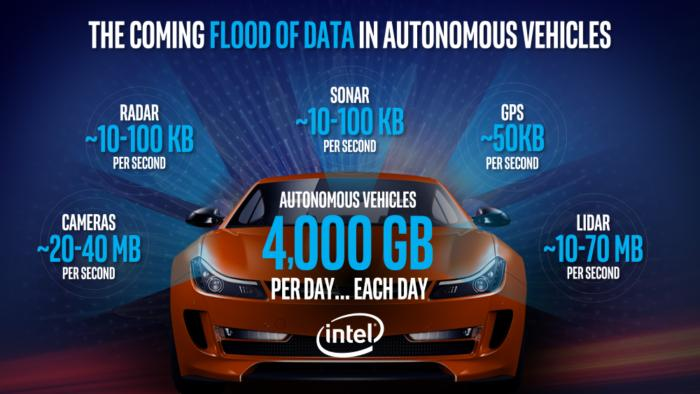
\includegraphics[scale=.5]{fig/autonomous-vehicle-data-intel-100697604-large.jpg}
\caption[Data Stats in Autonomous Cars]{Data Stats in Autonomous Cars\cite{datastats}}
\label{fig:datastats}
\end{center}
\end{figure}  
  
     \section{Motivation}	
For automotive applications, one major challenge is that all systems in the car should be real-time safe, that is, all systems of the car must give a guaranteed response within a specified time constraint. Missing a deadline can have disastrous consequences, such as, failure to apply the brakes at the right time after recognizing a person in front of the car may result in loss of life. 
One such software for communication data management is Robot Operating System(ROS). New versions of ROS, namely, ROS2 and micro-ROS offer support for real-time systems and embedded boards. The goal of this thesis is to test the real-time capability and robustness of ROS2 and micro-ROS under different test conditions.
	 \section{Objectives}
\begin{itemize}
  \item Research on state of the art
  \item Apply ROS2 concepts to explore Automotive Applications
  \item Set up STM32 microcontroller with RTOS and micro-ROS
  \item Test real-time performance of ROS2 using inverted pendulum demo  
  \item Test real-time performance of micro-ROS
  \item Analyzing results and documentation
\end{itemize}
	 

	 \section{Robot Operating System(ROS)}
	 {\bfseries ROS}
	 
The Robot Operating System (ROS) is a flexible framework for writing robot software. It is a collection of tools, libraries, and conventions that aim to simplify the task of creating complex and robust robot behavior across a wide variety of robotic platforms.\cite{ROS}	
It is an open-source software and is free to use for both research and commercial purposes.
 
But ROS does not guarantee deadlines and requires significant resources like high CPU\nomenclature{CPU}{Central Processing Unit} usage, high memory consumption, etc. Therefore, ROS is not suitable for resource constrained real-time systems.

{\bfseries	 ROS 2}

ROS 2 includes the components of ROS 1 which are great and improves those which are not.	ROS 2 was developed to satisfy new use cases like real-time systems, embedded systems, non-ideal networks, production environments, etc. It also uses new technologies like Data Distribution Service(DDS)\nomenclature{DDS}{Data Distribution Service}. The software is developed and maintained by Open Robotics.
It also offers support for different operating systems such as Linux, macOS, Microsoft Windows and different RTOSs. 
	 \clearpage
{\bfseries	 ROS 2 Distributions}
	 

The ROS 2 Distributions are shown below in descending order of release date. Dashing Diademata is the first long term support version offered by the ROS developers. The work in this thesis is based on the version Crystal Clemmys as the Dashing version was released in May, 2019 and enough documentation for real-time testing was not available for it. 

 
 

 
\includegraphics[scale=.112]{fig/eloquent-small.png} \hspace*{1cm}

\includegraphics[scale=.09]{fig/dashing-small.png}\hspace*{1cm}
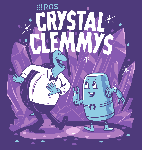
\includegraphics[scale=.48]{fig/crystal-small.png}\hspace*{1cm}
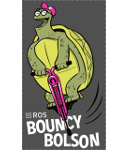
\includegraphics[scale=1]{fig/bouncy-small.png}\hspace*{1cm}

\includegraphics[scale=2]{fig/ardent-small.png}

\captionof{figure}[ROS 2 Distributions]{ROS 2 Distributions\cite{ROS2distro}}
\label{fig:ROS2Distro}

\vspace*{1cm}

{\bfseries	 micro-ROS}
\vspace*{0.5cm}

micro-ROS puts ROS 2 onto microcontrollers, making them first class participants of the ROS 2 environment.\cite{uros}	
It uses a real-time operating system(RTOS), here Nuttx by default, and DDS for eXtremely Resource Constrained Environments(DDS-XRCE)\nomenclature{DDS-XRCE}{DDS for eXtremely Resource Constrained Environments}. In this thesis, ROS 2 Crystal version is used with Nuttx RTOS on a STM32 microcontroller which is a 32-bit microcontroller by STMelectronics. This project is funded by Open Framework for Embedded Robot Applications(OFERA)\nomenclature{OFERA}{Open Framework for Embedded Robot Applications} consortium consisting of Bosch, eProsima, Acutronic Robotics, etc. 

\begin{figure}[ht]
\begin{center}

\includegraphics[scale=.3]{fig/microROS-big-logo.png}
\caption[micro-ROS Logo]{micro-ROS Logo\cite{uroslogo}}
\label{fig:uros}
\end{center}
\end{figure} 
	 
	\chapter{State of the Art}	
		
		
\rofoot[\pagemark]{\pagemark}
\refoot[\pagemark]{\pagemark}
	Real-time applications of ROS 2 have very recently come into the picture by the community. Many people have tested ROS 2 and have identified problems related to real-time performance. Also, the micro-ROS project is still in its infancy stage.
	
The core concepts of ROS 2, micro-ROS, embedded and real-time systems are mentioned in detail in this section. Also, the results of ROS 2 testing by some of the community members are stated.
	\section{ROS 2 Concepts}
	
	\vspace*{0.5cm}
	{\bfseries Node}
	
	
	\vspace*{0.5cm}
An executable/application that runs a program/subprogram that communicate with each other via streaming topics is known as a node.
It is used to communicate with other nodes using ROS client libraries which allow nodes to be written in different programming languages such as C, C++ and python. A robot may contain many nodes to control movement, analyse data, perform an operation like path planning, etc. 

In ROS 2, discovery of nodes is automatic through the underlying middleware. Nodes advertise information to other nodes when they go online, offline and also periodically for new nodes to join and enable communication. 


\vspace*{0.5cm}
	{\bfseries Topic}
	
	
	\vspace*{0.5cm}
	Topics are named buses over which nodes exchange messages. Topics have anonymous publish/subscribe semantics, which decouples the production of information from its consumption. In general, nodes are not aware of who they are communicating with. Instead, nodes that are interested in data subscribe to the relevant topic; nodes that generate data publish to the relevant topic. There can be multiple publishers and subscribers to a topic.\cite{topic}
	
	\vspace*{0.5cm}
	{\bfseries Message}
	
	
	\vspace*{0.5cm}
	Nodes communicate with each other by publishing messages to topics. A message is a simple data structure, comprising typed fields. Standard primitive types (integer, floating point, boolean, etc.) are supported, as are arrays of primitive types. Messages can include arbitrarily nested structures and arrays (much like C structs). msg files are simple text files for specifying the data structure of a message. These files are stored in the msg subdirectory of a package. Nodes can also exchange a request and response message as part of a ROS service call. These request and response messages are defined in srv files.\cite{messages}
	\begin{figure}[ht]
\begin{center}
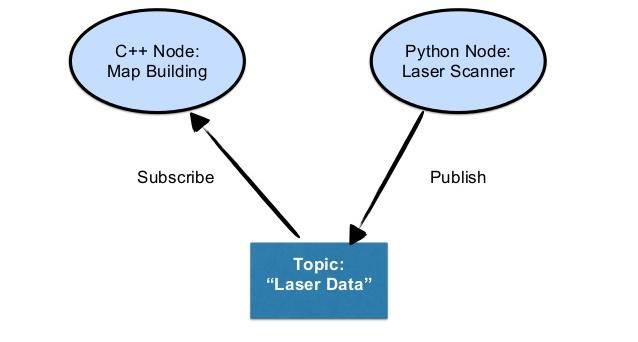
\includegraphics[scale=1]{fig/node_topic.jpg}
\caption[Working of Nodes, Topics and Messages]{Working of Nodes, Topics and Messages\cite{node_topic}}
\label{fig:node}
\end{center}
\end{figure}  
\vspace*{0.5cm}


	{\bfseries Data Distribution Service(DDS)}
	
	
	\vspace*{0.5cm}
	Data Distribution Service(DDS) is a middleware standard to ensure dependable,high performance, inter-operable,real-time data exchanges.Add more
	\vspace*{0.5cm}
	
	{\bfseries Quality of Service(QoS)\nomenclature{QoS}{Quality of Service}}
	
	
	\vspace*{0.5cm}
	

\vspace*{0.5cm}

	{\bfseries Executor}
	
	
\vspace*{0.5cm}
	\section{ROS 1 vs ROS 2}	
	
	\section{micro-ROS Architecture}

	\section{Embedded Systems}
	{\bfseries STM32 Micro-controller}
	{\bfseries Features}
	{\bfseries Communications  }
	{\bfseries IP}
	{\bfseries Serial}
	
	\section{Real-Time Systems}
	{\bfseries	Requirement}
	{\bfseries	Types : Soft}
	{\bfseries	Firm}
	{\bfseries	Hard}
	{\bfseries Pagefaults}	
	\section{Previous Research Results}

	\chapter{ADAS Applications using ROS 2}
		
\rofoot[\pagemark]{\pagemark}
\refoot[\pagemark]{\pagemark}
		\section{Lane Detection using Camera}
		\section{Auto Stop using LIDAR}
		\section{Driver Control using Keyboard}	
	
	
	
	\chapter{Test Setup}
		
\rofoot[\pagemark]{\pagemark}
\refoot[\pagemark]{\pagemark}

	\section{Testing micro-ROS}

	\subsection{Components}
	\subsection{Procedure}	

	\section{Testing ROS2}
	\subsection{Components}
	\subsection{Procedure}	


		\chapter{Results}
			
\rofoot[\pagemark]{\pagemark}
\refoot[\pagemark]{\pagemark}
		\section{Latency Analysis in micro-ROS}
		\section{Latency Analysis in ROS 2}
		
		
		\chapter{Conclusion and Future Scope}
			
\rofoot[\pagemark]{\pagemark}
\refoot[\pagemark]{\pagemark}
		\addcontentsline{toc}{chapter}{List of Figures}
	\listoffigures
	\addcontentsline{toc}{chapter}{List of Tables}
	\listoftables
		
		\addcontentsline{toc}{chapter}{Bibliography}
\bibliographystyle{ieeetr}		
\bibliography{thesis}





\end{document}
